\documentclass[tikz]{standalone}
\usepackage{amsmath}
\usetikzlibrary{calc}
\definecolor{acc}{HTML}{F7B538}
\definecolor{bg}{HTML}{171D2B}
\definecolor{tri1}{HTML}{5B8DEF}
\definecolor{tri2}{HTML}{34C98E}
\pagecolor{bg}
\begin{document}
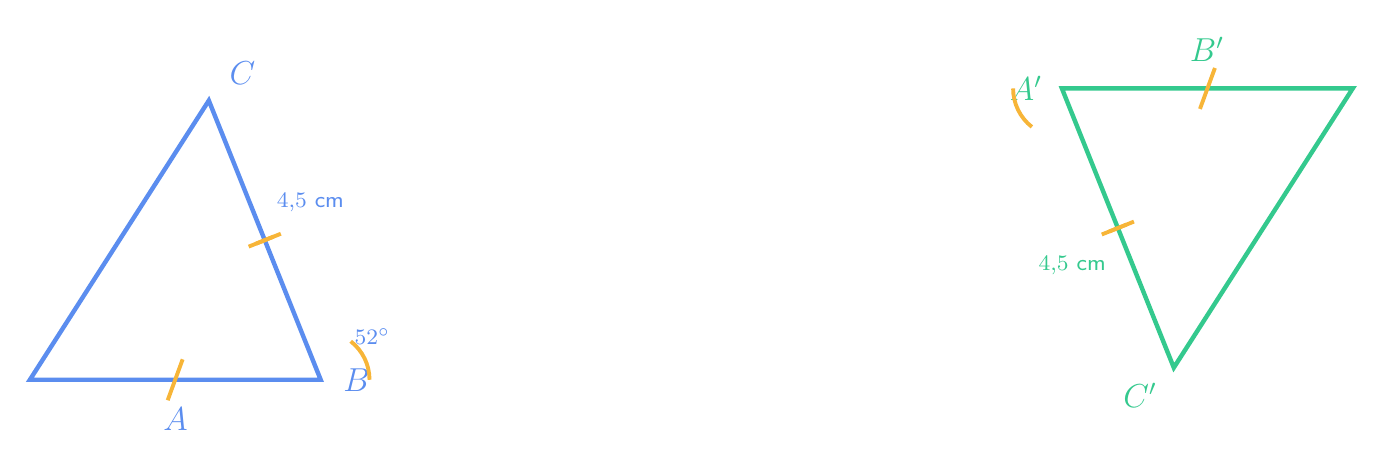
\begin{tikzpicture}[
  line width=1.6pt,
  every node/.style={text=white, font=\sffamily\large},
  tickmark/.style={line width=1.4pt, draw=acc},
  anglemark/.style={line width=1.4pt, draw=acc}
]
% ===== Segitiga ABC (biru): AB=6, BC=4.5, sudut B=52 derajat =====
\coordinate (A) at (0,0);
\coordinate (B) at (3.6933,0);
\coordinate (C) at (2.2724,3.5460);
\draw[tri1] (A) -- (B) -- (C) -- cycle;
\node[tri1] at (1.85,-0.5) {$A$};
\node[tri1] at (4.15,0.0) {$B$};
\node[tri1] at (2.7,3.9) {$C$};
% tanda satu garis pada AB
\draw[tickmark] (1.75,-0.26) -- (1.94,0.26);
% tanda dua garis pada BC
\coordinate (Mbc) at ($(B)!0.5!(C)$);
\draw[tickmark] ($(Mbc)!0.12cm!90:(B)$) -- ($(Mbc)!0.12cm!90:(C)$);
\draw[tickmark] ($(Mbc)!0.22cm!90:(B)$) -- ($(Mbc)!0.22cm!90:(C)$);
% busur sudut B
\draw[anglemark] (B) ++(52:0.62) arc[start angle=52, end angle=0, radius=0.62];
\node[tri1] at (4.35,0.55) {\footnotesize $52^\circ$};
% label panjang
\node at (1.85,0.35) {\footnotesize $6$ cm};
\node[tri1] at ($(B)!0.62!(C)+(0.75,0.05)$) {\footnotesize $4{,}5$ cm};
% ===== Segitiga A'B'C' (hijau), kongruen, diputar 180 =====
\begin{scope}[rotate around={180:(8.4,1.85)}]
  \coordinate (A2) at (0,0);
  \coordinate (B2) at (3.6933,0);
  \coordinate (C2) at (2.2724,3.5460);
  \draw[tri2] (A2) -- (B2) -- (C2) -- cycle;
  \node[tri2] at (1.85,-0.5) {$B'$};
  \node[tri2] at (4.15,0.0) {$A'$};
  \node[tri2] at (2.7,3.9) {$C'$};
  % tanda satu garis pada A'B'
  \draw[tickmark] (1.75,-0.26) -- (1.94,0.26);
  % tanda dua garis pada A'C'
  \coordinate (Mac) at ($(B2)!0.5!(C2)$);
  \draw[tickmark] ($(Mac)!0.12cm!90:(B2)$) -- ($(Mac)!0.12cm!90:(C2)$);
  \draw[tickmark] ($(Mac)!0.22cm!90:(B2)$) -- ($(Mac)!0.22cm!90:(C2)$);
  % busur sudut A'
  \draw[anglemark] (B2) ++(52:0.62) arc[start angle=52, end angle=0, radius=0.62];
  % label panjang
  \node at (1.85,0.35) {\footnotesize $6$ cm};
  \node[tri2] at ($(B2)!0.62!(C2)+(0.75,0.05)$) {\footnotesize $4{,}5$ cm};
\end{scope}
\end{tikzpicture}
\end{document}
